\documentclass{beamer}
\usepackage{amsmath}
\usepackage[english]{babel} %set language; note: after changing this, you need to delete all auxiliary files to recompile
\usepackage[utf8]{inputenc} %define file encoding; latin1 is the other often used option
\usepackage{csquotes} % provides context sensitive quotation facilities
\usepackage{graphicx} %allows for inserting figures
\usepackage{booktabs} % for table formatting without vertical lines
\usepackage{textcomp} % allow for example using the Euro sign with \texteuro
\usepackage{stackengine}
\usepackage{wasysym}
\usepackage{tikzsymbols}
\usepackage{textcomp}
\usepackage{xcolor}
\usepackage[dvipsnames]{xcolor}
\usepackage{colortbl}
\usepackage{adjustbox}
\usepackage{tikz}
\usepackage{pgfplots}
\pgfplotsset{compat=1.18}
\usetikzlibrary{arrows.meta, calc, decorations.pathreplacing}


\usepackage{amssymb}
\usepackage{multirow}

% Colores
\definecolor{rojo}{RGB}{221, 36, 36}
\definecolor{celeste}{RGB}{173, 216, 230}

\newcommand{\up}{\textcolor{blue}{\Large$\uparrow$}}
\newcommand{\down}{\textcolor{red}{\Large$\downarrow$}}
\newcommand{\question}{\textcolor{red}{\Large\textbf{?}}}


% ELIMINAR COMANDOS DE NAVEGACION%%%%%%%%%%%
\setbeamertemplate{navigation symbols}

%\newcommand{\bubblethis}[2]{
 %       \tikz[remember picture,baseline]{\node[anchor=base,inner sep=0,outer sep=0]%
 %       (#1) {\underline{#1}};\node[overlay,cloud callout,callout relative pointer={(0.2cm,-0.7cm)},%
 %       aspect=2.5,fill=yellow!90] at ($(#1.north)+(-0.5cm,1.6cm)$) {#2};}%
 %   }%
%\tikzset{face/.style={shape=circle,minimum size=4ex,shading=radial,outer sep=0pt,
 %       inner color=white!50!yellow,outer color= yellow!70!orange}}

%% Some commands to make the code easier
\newcommand{\emoticon}[1][]{%
  \node[face,#1] (emoticon) {};
  %% The eyes are fixed.
  \draw[fill=white] (-1ex,0ex) ..controls (-0.5ex,0.2ex)and(0.5ex,0.2ex)..
        (1ex,0.0ex) ..controls ( 1.5ex,1.5ex)and( 0.2ex,1.7ex)..
        (0ex,0.4ex) ..controls (-0.2ex,1.7ex)and(-1.5ex,1.5ex)..
        (-1ex,0ex)--cycle;}
\newcommand{\pupils}{
  %% standard pupils
  \fill[shift={(0.5ex,0.5ex)},rotate=80] 
       (0,0) ellipse (0.3ex and 0.15ex);
  \fill[shift={(-0.5ex,0.5ex)},rotate=100] 
       (0,0) ellipse (0.3ex and 0.15ex);}

\newcommand{\emoticonname}[1]{
  \node[below=1ex of emoticon,font=\footnotesize,
        minimum width=4cm]{#1};}
\usepackage{scalerel}
\usetikzlibrary{positioning}
\usepackage{xcolor,amssymb}
\newcommand\dangersignb[1][2ex]{%
  \scaleto{\stackengine{0.3pt}{\scalebox{1.1}[.9]{%
  \color{red}$\blacktriangle$}}{\tiny\bfseries !}{O}{c}{F}{F}{L}}{#1}%
}
\newcommand\dangersignw[1][2ex]{%
  \scaleto{\stackengine{0.3pt}{\scalebox{1.1}[.9]{%
  \color{red}$\blacktriangle$}}{\color{white}\tiny\bfseries !}{O}{c}{F}{F}{L}}{#1}%
}
\usepackage{fontawesome} % Social Icons
\usepackage{epstopdf} % allow embedding eps-figures
\usepackage{tikz} % allows drawing figures
\usepackage{amsmath,amssymb,amsthm} %advanced math facilities
\usepackage{lmodern} %uses font that support italic and bold at the same time
\usepackage{hyperref}
\usepackage{tikz}
\hypersetup{
    colorlinks=true,
    linkcolor=blue,
    filecolor=magenta,      
    urlcolor=blue,
}
\usepackage{tcolorbox}
%add citation management using BibLaTeX
\usepackage[citestyle=authoryear-comp, %define style for citations
    bibstyle=authoryear-comp, %define style for bibliography
    maxbibnames=10, %maximum number of authors displayed in bibliography
    minbibnames=1, %minimum number of authors displayed in bibliography
    maxcitenames=3, %maximum number of authors displayed in citations before using et al.
    minnames=1, %maximum number of authors displayed in citations before using et al.
    datezeros=false, % do not print dates with leading zeros
    date=long, %use long formats for dates
    isbn=false,% show no ISBNs in bibliography (applies only if not a mandatory field)
    url=false,% show no urls in bibliography (applies only if not a mandatory field)
    doi=false, % show no dois in bibliography (applies only if not a mandatory field)
    eprint=false, %show no eprint-field in bibliography (applies only if not a mandatory field)
    backend=biber %use biber as the backend; backend=bibtex is less powerful, but easier to install
    ]{biblatex}
\addbibresource{../mybibfile.bib} %define bib-file located one folder higher


\usefonttheme[onlymath]{serif} %set math font to serif ones

\definecolor{beamerblue}{rgb}{0.2,0.2,0.7} %define beamerblue color for later use

%%% defines highlight command to set text blue
\newcommand{\highlight}[1]{{\color{blue}{#1}}}


%%%%%%% commands defining backup slides so that frame numbering is correct

\newcommand{\backupbegin}{
   \newcounter{framenumberappendix}
   \setcounter{framenumberappendix}{\value{framenumber}}
}
\newcommand{\backupend}{
   \addtocounter{framenumberappendix}{-\value{framenumber}}
   \addtocounter{framenumber}{\value{framenumberappendix}}
}

%%%% end of defining backup slides

%Specify figure caption, see also http://tex.stackexchange.com/questions/155738/caption-package-not-working-with-beamer
\setbeamertemplate{caption}{\insertcaption} %redefines caption to remove label "Figure".
%\setbeamerfont{caption}{size=\scriptsize,shape=\itshape,series=\bfseries} %sets figure  caption bold and italic and makes it smaller


\usetheme{Boadilla}

%set options of hyperref package
\hypersetup{
    bookmarksnumbered=true, %put section numbers in bookmarks
    naturalnames=true, %use LATEX-computed names for links
    citebordercolor={1 1 1}, %color of border around cites, here: white, i.e. invisible
    linkbordercolor={1 1 1}, %color of border around links, here: white, i.e. invisible
    colorlinks=true, %color links
    anchorcolor=black, %set color of anchors
    linkcolor=beamerblue, %set link color to beamer blue
    citecolor=blue, %set cite color to beamer blue
    pdfpagemode=UseThumbs, %set default mode of PDF display
    breaklinks=true, %break long links
    pdfstartpage=1 %start at first page
    }

\newtcolorbox{boxA}{
    fontupper = \bf,
    boxrule = 1.5pt,
    colframe = black % frame color
}
\newtcolorbox{boxB}{
    boxrule = 1.5pt,
    colframe = blue!70!black,, % frame color
    colback = blue!7!white,
}

% --------------------
% Overall information
% --------------------
\title[Economía I]{Economía I \vspace{3mm}
\\ Magistral 14 \vspace{3mm} \\ Repaso}
\date{}
\author[Victoria Rosino]{Victoria Rosino}
\vspace{0.3cm}
\institute[]{Universidad de San Andrés} 

\begin{document}

\begin{frame}
\vspace{0.3cm}
\titlepage
\centering
\vspace{-0.9cm}

\includegraphics[scale=0.3]{Slides Principios de Economia/Figures/udesa_logo.jpg} 
\end{frame}



\begin{frame}{Ejercicio 1: Mercado de remeras ilustradas}

En el mercado de remeras ilustradas, la demanda y la oferta están dadas por las siguientes funciones:

\begin{itemize}
    \item Demanda: $Q_d = 1400 - 2P$
    \item Oferta: $Q_o = P-100$
\end{itemize}

Donde $Q$ representa la cantidad de remeras por mes y $P$ el precio por unidad en pesos.
\end{frame}

\begin{frame}{Preguntas}

\begin{enumerate}
    \item Grafique la curva de demanda y de oferta en un mismo gráfico.
    \item Calcule el precio y la cantidad de equilibrio.
    \item Calcule el \textbf{excedente del consumidor} y el \textbf{excedente del productor} en equilibrio.
    \item Calcule la \textbf{elasticidad-precio de la demanda} y la \textbf{elasticidad-precio de la oferta} 
    \item Calcule la \textbf{elasticidad-precio de la demanda} en el punto de equilibrio si el precio baja un 10\%, usando el \textbf{método del punto medio}.
    \item Analice qué ocurre si la demanda se reduce: $Q_d = 1000 - 2P$ 
        \begin{itemize}
            \item  ¿Qué sucede con el precio y la cantidad de equilibrio ? 
            \item Identifique posibles causas de este cambio.
            \item ¿Qué sucede los excedentes? 
        \end{itemize}
\end{enumerate}
\end{frame}

\begin{frame}{Resolución: Equilibrio inicial}
\textbf{Igualamos demanda y oferta:}

\begin{align*}
1400 - 2P &= P -100 \\
1500 &= 3P \Rightarrow P^* = 500
\end{align*}

\textbf{Sustituimos en la oferta:}
\[
Q^* = 500 - 100 = 400
\]

\textbf{Equilibrio inicial:} Precio = \$500, Cantidad = 400 remeras.
\end{frame}

\begin{frame}{Resolución: Excedentes en equilibrio inicial}
\textbf{Excedente del consumidor (EC):} \\
Precio máximo dispuesto a pagar: $Q_d = 0 \Rightarrow 1400 - 2P = 0 \Rightarrow P = 700$

\[
EC = \frac{(700 - 500) \cdot 400}{2}  = \frac{200\cdot 200}{2}  = \textbf{40.000}
\]

\textbf{Excedente del productor (EP):} \\
Precio mínimo aceptado: $Q_o = 0 \Rightarrow P-100 = 0 \Rightarrow P = 100$

\[
EP = \frac{(500-100) \cdot400 }{2} = \frac{400 \cdot 400}{2} = \textbf{80.000}
\]
\end{frame}
\begin{frame}{Resolución: Elasticidad}
\textbf{Elasticidad puntual de la demanda en el equilibrio:}
\[
\varepsilon = \left| \frac{\Delta Q}{\Delta P} \cdot \frac{P^*}{Q^*} \right| = \left| -2 \cdot \frac{500}{400} \right| = 2,5
\]

\textbf{Elasticidad puntual de la oferta en el equilibrio:}
\[
\varepsilon = \frac{\Delta Q}{\Delta P} \cdot \frac{P^*}{Q^*}  = 1 \cdot \frac{500}{400}  = 1,25
\]

\textbf{Elasticidad con el método del punto medio:} \\
Si el precio baja 10\%: $P_1 = 500 \Rightarrow P_2 = 450$, entonces:

\[
Q_1 = 1400 - 2 \cdot 500 = 400 \qquad Q_2 = 1400 - 2 \cdot 450 = 500
\]

\[
\varepsilon = \left| \frac{Q_2 - Q_1}{P_2 - P_1} \cdot \frac{\frac{P_1 + P_2}{2}}{\frac{Q_1 + Q_2}{2}} \right| = \left| \frac{100}{-50} \cdot \frac{950}{900} \right| = \left| -2 \cdot 1,05 \right| \approx 2,11
\]
\end{frame}

\begin{frame}{Análisis del cambio}
\begin{itemize}
    \item El precio cayó de \$500 a \$366,6.
    \item La cantidad cayó de 400 a 266 (aprox.) remeras.
    \item El \textbf{excedente del consumidor} disminuyó.
    \item El \textbf{excedente del productor} también disminuyó.
    \item Esto puede deberse, por ejemplo, a:
        \begin{itemize}
            \item Menor interés del público en las remeras (cambio en las preferencias).
            \item Caída en el ingreso
            \item Caída del precio de las chombas (sustituto)
        \end{itemize}
\end{itemize}
\end{frame}

\begin{frame}{Ejercicio 2: Efecto Sustitución y Efecto Ingreso}
    \scriptsize
    Suponga que Julia consume únicamente dos bienes: Pizza (bien X) y Entradas al Cine (bien Y). Julia tiene un ingreso semanal de \$600. El precio inicial de una pizza es \$30 y el precio inicial de una entrada al cine es \$20. Actualmente, Julia elige consumir 10 pizzas y 15 entradas al cine cada semana.
    Debido a una reducción en el precio de la pizza, ahora cada pizza cuesta solo \$20, manteniéndose constante tanto el precio del cine (\$20) como el ingreso semanal de Julia (\$600). Tras esta reducción en el precio, Julia modifica su consumo y ahora compra 15 pizzas y 15 entradas al cine.
    \begin{enumerate}
        \item Dibuje cuidadosamente el gráfico presupuestario original y el nuevo tras la reducción en el precio de la pizza. Indique claramente los interceptos y la pendiente en ambos casos. Indique el punto inicial y final del consumo de Julia.
        \item Indique gráficamente cómo se descompone el cambio total en dos componentes: efecto sustitución y efecto ingreso. Responda:
        \begin{itemize}
            \scriptsize
            \item ¿Qué significa el efecto sustitución para el consumo de pizza? ¿Cómo se relaciona con el efecto sustitución en el consumo de entradas al cine?
            \item ¿Qué significa el efecto ingreso para el consumo de pizza? ¿Cómo se relaciona con el efecto ingreso en el consumo de entradas al cine?
        \end{itemize}
    \end{enumerate}
\end{frame}

\begin{frame}
\frametitle{Ejercicio 2: Efecto Sustitución y Efecto Ingreso}
\begin{center}
\begin{figure}[H]
\renewcommand{\figurename}{Figure}
\begin{center}
\begin{tikzpicture}[scale=0.8]
\draw[very thick,<->] (0,7.5) node[left]{Cine}--(0,0)--(9,0) node[below]{Pizza};

\only<2->{
\draw [thick] (0,6) -- (4,0);
\draw [thick] (1.35,4.7) to [out=280,in=170] (4,1.8);
\node[below] at (4,0) {\footnotesize 20};
\node[left] at (0,3) {\footnotesize 15};
\node[below] at (2,0) {\footnotesize 10};
\node[left] at (0,6) {\footnotesize 30};
\node [right] at (2,3) {\footnotesize $A$};
\draw[fill] (2,3) circle [radius =0.06];
\draw[thin, dashed,gray](2,0)--(2,3);
\draw[thin, dashed,gray](0,3)--(2,3);
}

\only<3->{
\draw [thick, blue] (0,6) -- (6,0);
\draw [thick] (1.97,5.15) to [out=280,in=170] (4.5,2.3);
\node[below] at (3,0) {\footnotesize 15};
\node[below] at (6,0) {\footnotesize 30};
\node [right] at (3,3.12) {\footnotesize $B$};
\draw[fill] (3,3.03) circle [radius =0.06];
\draw[thin, dashed,gray](3,0)--(3,3);
\draw[thin, dashed,gray](2,3)--(3,3);

}

\only<4->{
\draw[thin, dashed,gray](2.6,0)--(2.6,3.47);
\draw[thin, dashed,gray](0,3.47)--(2.6,3.47);
\draw [thick, red!30] (0.215,7) -- (4.92,0);
\node [above right] at (2.6,3.47) {\footnotesize $C$};
\draw[fill] (2.6,3.47) circle [radius =0.06];
}

\only<5->{

%\draw[semithick, blue, <-] (1,-1)--(3.2,-1);
%\node[] at (1.7,-1.2){\tiny Efecto};
%\node[] at (2.4,-1.2){\tiny Total};

\draw[semithick, blue, ->] (1.9,-0.65)--(2.6,-0.65);
\node[] at (2.3,-0.85){\tiny EI};
\draw[semithick, blue, ->] (2.65,-0.65)--(3.1,-0.65);
\node[] at (2.8,-0.85){\tiny ES};


\draw[semithick, blue, ->] (-0.65,3)--(-0.65,3.5);
\node[] at (-0.9,3.2){\tiny EI};
\draw[semithick, blue, <-] (-1.2,3)--(-1.2,3.5);
\node[] at (-1.5,3.2){\tiny ES};


}

\end{tikzpicture}
\end{center}
\end{figure}
\end{center}
\end{frame}

\begin{frame}
\frametitle{Ping Pong de Verdaderos/Falsos}
\centering

Cuando el productor puede apropiarse de todo lo que genera, trabajará hasta el punto en que la producción marginal que obtiene se iguale con el ingreso adicional necesario para cubrir sus necesidades básicas

\end{frame}

\begin{frame}{Ping Pong de Verdaderos/Falsos}
    \centering
    \tiny
    \begin{figure}[h!]
        \renewcommand{\figurename}{Figure}
        \begin{center}
        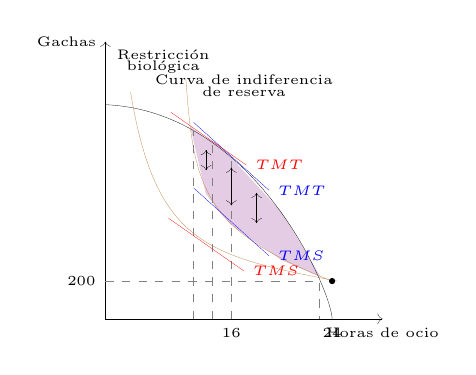
\begin{tikzpicture}[scale=0.32]
        \draw[fill,violet!20] (3.4,7.6)--(4,5)--(4.5,4.3)--(5,3.75)--(7,2.35)--(8.5,1.7)--(7,4.2)--(4.5,6.9)--(4,7.15);
        \draw[ultra thin,<->] (0,11) node[left]{\fontsize{5pt}{5pt}\selectfont Gachas}--(0,0)--(11,0) node[below]{\fontsize{5pt}{5pt}\selectfont Horas de ocio};
        
        \draw[ultra thin, brown] (1,9).. controls (2,3) and (4, 2.5) .. (9.2, 1.5);
        \draw[ultra thin] (0,8.5).. controls (6,8.25) and (9, 1) .. (9,0);

     \draw[ultra thin, brown] (3.2,9.5).. controls (3.5,5) and (4, 3.5) .. (9, 1.5);
        
        \draw[ultra thin, dashed, gray] (0,1.5)--(8.5,1.5)--(8.5,0);
        % \draw[ultra thin, dashed, gray] (1.05,0)--(1.05,8.25);
        \draw[ultra thin, dashed, gray] (3.5,0)--(3.5,7.5);
        \draw[ultra thin, dashed, gray] (4.25,0)--(4.25,7);
        \draw[ultra thin, dashed, gray] (5,0)--(5,6.4);
        % \node[below] at (1.05,0) {{\fontsize{4pt}{4pt}\selectfont $4$};
        \node[below] at (5,0) {\fontsize{4pt}{4pt}\selectfont $16$};
        \node[left] at (0,1.5) {\fontsize{4pt}{4pt}\selectfont $200$};
        \draw[fill] (9,1.5) circle [radius =0.1];
        \node[below] at (9,0) {\fontsize{5pt}{5pt}\selectfont $24$};
        \draw[ultra thin, blue] (3.5,7.8)--(6.5,5.1) node[right]{\fontsize{4pt}{4pt}\selectfont $TMT$};
        \draw[ultra thin, blue] (3.5,5.2)--(6.5,2.5) node[right]{\fontsize{4pt}{4pt}\selectfont $TMS$};
        \node[] at (5.5,9.5) {\fontsize{4pt}{4pt}\selectfont Curva de indiferencia};
        \node[] at (5.5,9) {\fontsize{4pt}{4pt}\selectfont  de reserva};
        \node[] at (2.3,10.5) {\fontsize{4pt}{4pt}\selectfont Restricción};
        \node[] at (2.3,10) {\fontsize{4pt}{4pt}\selectfont  biológica};
        \draw[ultra thin, <->] (5,4.5)--(5,6);
        \draw[ultra thin, <->] (6,3.8)--(6,5);
        \draw[ultra thin, <->] (4,5.9)--(4,6.7);
        \draw[ultra thin, red] (2.6,8.2)--(5.6,6.1) node[right]{\fontsize{4pt}{4pt}\selectfont $TMT$};
        \draw[ultra thin, red] (2.5,4)--(5.5,1.9) node[right]{\fontsize{4pt}{4pt}\selectfont $TMS$};
        \end{tikzpicture}
        
        \begin{tikzpicture}[scale=0.32]
        \draw[ultra thin,<->] (0,11) node[left]{\fontsize{5pt}{5pt}\selectfont Gachas}--(0,0)--(11,0) node[below]{\fontsize{5pt}{5pt}\selectfont Horas de ocio};
        \draw[ultra thin, dashed, gray] (3.5,0)--(3.5,11.5);
        \draw[ultra thin, dashed, gray] (8.5,0)--(8.5,11.5);
        \draw[ultra thin, dashed, gray] (4.25,0)--(4.25,11.5);
        \draw[ultra thin, dashed, gray] (5,0)--(5,11.5);
        \draw[ultra thin, violet] (3.5,0).. controls (4,3.5) and (6,4) .. (8.5, 0);
        \draw[ultra thin, <->] (4,0.25)--(4,1.2);
        \draw[ultra thin, <->] (5,0.25)--(5,2);
        \draw[ultra thin, <->] (6,0.25)--(6,1.2);
        \end{tikzpicture}
        \end{center}
    \end{figure}
\end{frame}


\begin{frame}
\frametitle{Ping Pong de Verdaderos/Falsos}
    \centering

    La servidumbre con porcentaje de producción garantiza eficiencia porque permite al dueño de la tierra participar de los beneficios sin eliminar el incentivo del productor.

\end{frame}

\begin{frame}{Ping Pong de Verdaderos/Falsos}
    \centering
    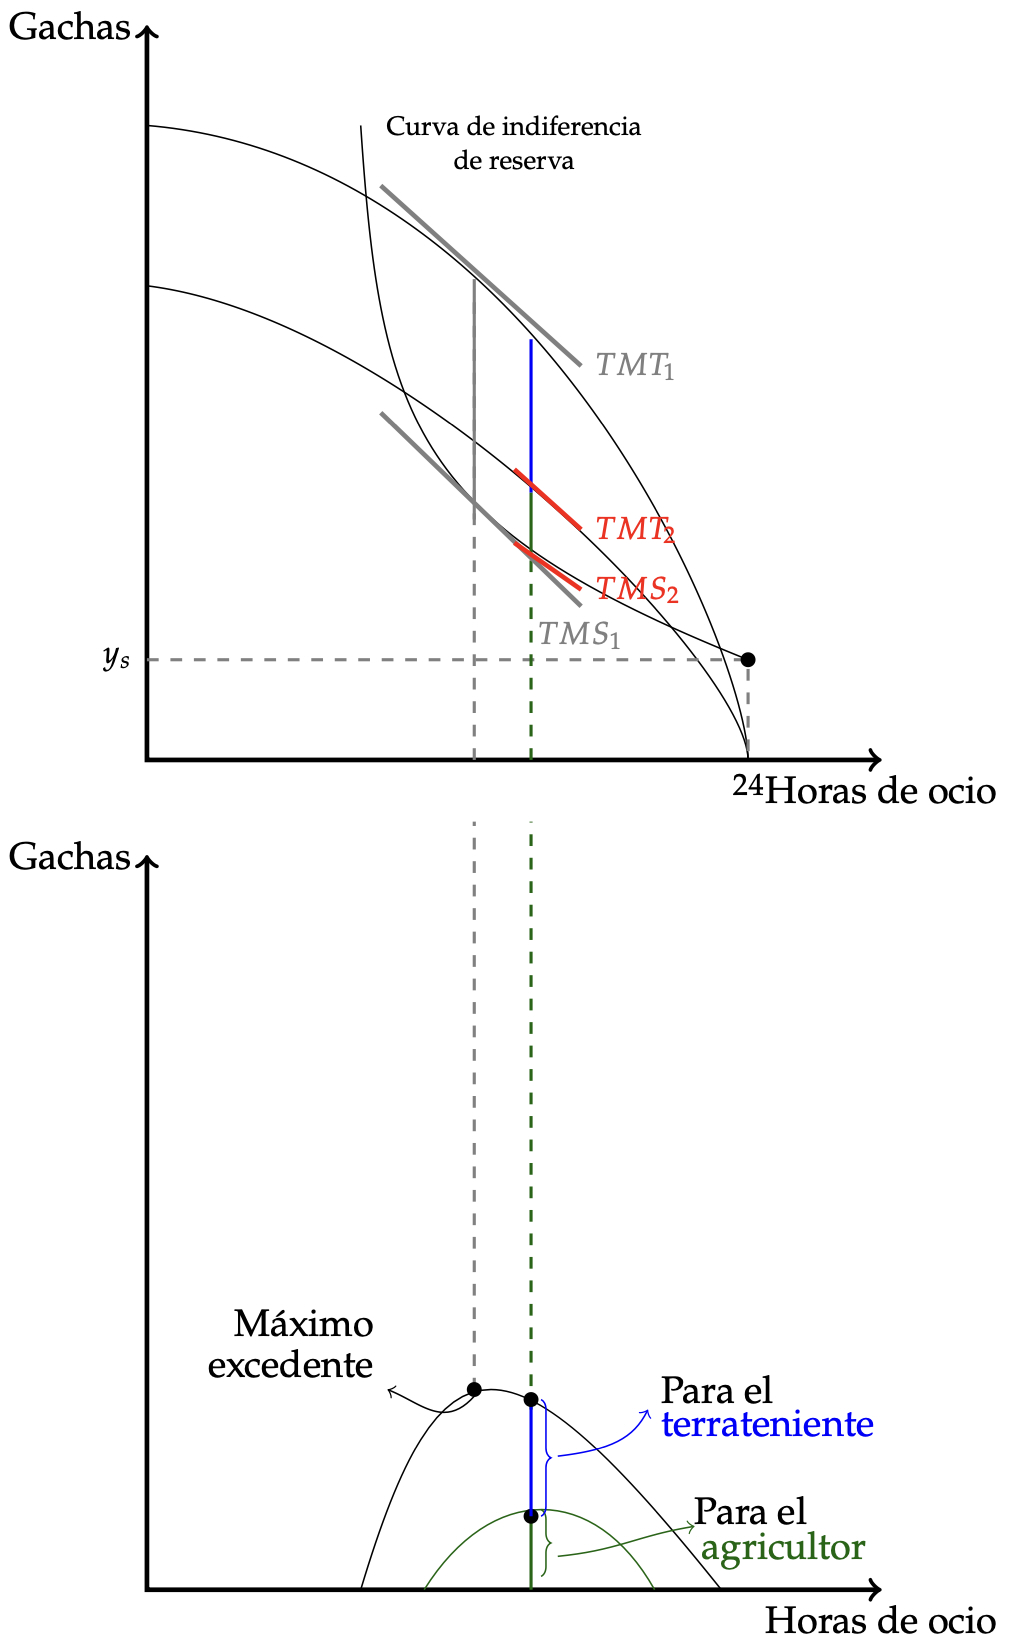
\includegraphics[scale=0.28]{Slides Principios de Economia/Figures/Magistral_09/C19.15.jpg}
\end{frame}

\begin{frame}
\frametitle{Ping Pong de Verdaderos/Falsos}
    \centering
    El modelo institucional sugiere que los malos resultados económicos no siempre se deben a falta de tecnología, sino a reglas que desincentivan el esfuerzo.
\end{frame}


\begin{frame}
\frametitle{Ping Pong de Verdaderos/Falsos}
\centering
Lucía consume chocolate y helado. En su punto de consumo actual, está dispuesta a dar 3 helados por una barra de chocolate. Si en el mercado el chocolate cuesta 4 veces más que el helado, Lucía no está en un punto óptimo y debería consumir más helado.
\end{frame}

\begin{frame}{Ping Pong de Verdaderos/Falsos}
    \centering
    La diferencia entre el costo medio total y el costo medio variable es constante, porque los costos fijos no cambian con la cantidad producida.
\end{frame}

\begin{frame}{Ping Pong de Verdaderos/Falsos}
    \centering
    Cuando el costo medio variable es creciente, necesariamente el costo marginal es menor al costo medio variable.
\end{frame}


\begin{frame}{Ping Pong de Verdaderos/Falsos}
    \centering
    La empresa Whirlpool produce heladeras y se enfrenta a una competencia fuerte. La empresa tiene una elasticidad cruzada con respecto al precio al que vende la empresa Electrolux de 0,5 y una elasticidad cruzada del precio al que vende la empresa LG de 1,2. Esto implica que Whirlpool prefiere que Electrolux baje sus precios.
\end{frame}




\end{document}
